\documentclass[lang=cn, chinesefont=founder, color=cyan, citestyle=gb7714-2015, bibstyle=gb7714-2015]{elegantbook}

\usepackage{unicode-math}
\setmathfont{STIXTwoMath-Regular.otf}

\usepackage[color=black]{siunitx}
\usepackage{tikz}
\usepackage{tkz-euclide}
\usepackage{tkz-graph}
\usepackage{dashrule}
\usepackage{float}

\PassOptionsToPackage{dvipsnames,svgnames,x11names}{xcolor}

\definecolor{shadow}{RGB}{210,241,241}

\tcbuselibrary{minted}
\newcommand{\spare}{\vspace{-1em}\begin{center}\color{structurecolor}\hdashrule[0.5ex]{\textwidth}{1pt}{1pt}\end{center}\vspace{-1em}}
\usetikzlibrary{shapes,backgrounds}
\ExecuteBibliographyOptions{sorting=gb7714-2015}
\setlength{\parskip}{1ex}
\newtcolorbox{collections}{
      boxrule=0.5pt,
      enhanced,
      breakable,
      top=8pt,
      before skip=8pt,
      colframe=structurecolor,
      colback=structurecolor!5,
      colbacktitle=structurecolor
}
\newtcblisting{code}[1]{
    listing engine=minted,
    boxrule=0.1mm,
    colback=third!5,
    colframe=third,
    listing only,
    left=5mm,
    enhanced,
    breakable,
    overlay={\begin{tcbclipinterior}\fill[third] (frame.south west)
    rectangle ([xshift=5mm]frame.north west);\end{tcbclipinterior}},
    minted language=#1,
    minted style=xcode,
    minted options={breaklines, mathescape, autogobble, linenos, numbersep=2mm}
}
\renewcommand{\theFancyVerbLine}{\textcolor{white}{\footnotesize{\arabic{FancyVerbLine}}}}

\renewcommand{\bar}[1]{\overline{#1}}
\renewcommand\arraystretch{1.2}
\arrayrulecolor{second}

\usetikzlibrary{graphs}

\title{新世代计算机科学计划·基础篇}
\author{JouderMin}
\institute{「新世代计算机科学计划」制作委员会}
\date{\zhtoday}
\cover{img/cover.png}
\logo{img/方形logo.png}

\begin{document}
\maketitle
\frontmatter

\tableofcontents

\mainmatter

\chapter{离散数学}
\input{SectionPage/1.1.tex}
\input{SectionPage/1.2.tex}

\section{图的概念}
\begin{introduction}
    \item 图
    \item 无向图、有向图与混合图
    \item 环、多重边
    \item 简单图、伪图与多重图
    \item 完全图、零图与平凡图
    \item 顶点与边的性质
    \item 子图与并图
\end{introduction}

\subsection{图}
图是由顶点与连接顶点的边构成的离散结构,图的定义如下
\begin{definition}[图]\label{def:图}
    图 $G = (V, E)$ 由顶点的非空集 $V$ 和边集 $E$ 构成,每条边有一个或两个顶点与之相连,这样的顶点叫做边的端点。
\end{definition}

图 \ref{fig:图} 展示了一个图。
\begin{figure}[H]
    \centering
    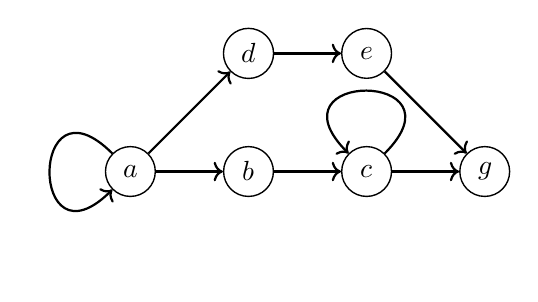
\begin{tikzpicture}
        \GraphInit[vstyle=normal]
        \SetGraphUnit{1.5}
        \Vertex[Math=true]{a}
        \EA[Math=true](a){b}
        \EA[Math=true](b){c}
        \EA[Math=true](c){g}
        \NO[Math=true](b){d}
        \NO[Math=true](c){e}
        \Edge[style={->}](a)(b)
        \Edge[style={->}](b)(c)
        \Edge[style={->}](c)(g)
        \Edge[style={->}](a)(d)
        \Edge[style={->}](d)(e)
        \Edge[style={->}](e)(g)
        \Loop[dist=1.5cm, style={->}](a)
        \Loop[dist=1.5cm, dir=NO, style={->}](c)
    \end{tikzpicture}
    \caption{图}
    \label{fig:图}
\end{figure}

\subsection{无向图、有向图与混合图}
图可以根据边是否有方向这一特性来划分为无向图、有向图与混合图三类。
\begin{definition}[有向边与无向边]\label{def:无向边与有向边}
    无向边以基数为 2 的集合表示,$\{u, v\}$ 表示该无向边与顶点 $u$、$v$ 相关联。有向边以序偶表示,$(u, v)$ 表示该有向边与顶点 $u$、$v$ 相关联,且开始于 $u$,结束于 $v$。
\end{definition}

由此,如果图 $G$ 的边集 $E$ 中只有无向边,则该图称为无向图;如果图 $G$ 的边集 $E$ 中只有有向边,则该图称为有向图;如果图 $G$ 的边集 $E$ 中同时存在无向边与有向边,则该图称为混合图。
\begin{figure}[H]
    \centering
    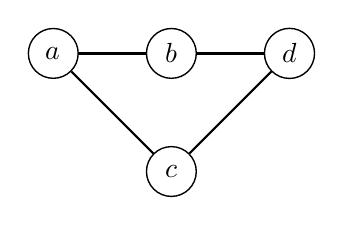
\begin{tikzpicture}
        \GraphInit[vstyle=normal]
        \SetGraphUnit{1.5}
        \Vertex[Math=true]{a}
        \EA[Math=true](a){b}
        \SO[Math=true](b){c}
        \EA[Math=true](b){d}
        \Edge[style={-}](a)(b)
        \Edge[style={-}](a)(c)
        \Edge[style={-}](b)(d)
        \Edge[style={-}](c)(d)
    \end{tikzpicture}
    \hspace{1em}
    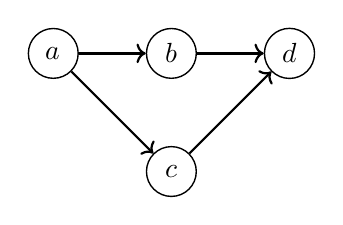
\begin{tikzpicture}
        \GraphInit[vstyle=normal]
        \SetGraphUnit{1.5}
        \Vertex[Math=true]{a}
        \EA[Math=true](a){b}
        \SO[Math=true](b){c}
        \EA[Math=true](b){d}
        \Edge[style={->}](a)(b)
        \Edge[style={->}](a)(c)
        \Edge[style={->}](b)(d)
        \Edge[style={->}](c)(d)
    \end{tikzpicture}
    \hspace{1em}
    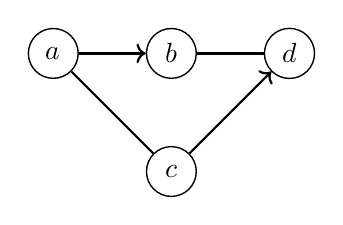
\begin{tikzpicture}
        \GraphInit[vstyle=normal]
        \SetGraphUnit{1.5}
        \Vertex[Math=true]{a}
        \EA[Math=true](a){b}
        \SO[Math=true](b){c}
        \EA[Math=true](b){d}
        \Edge[style={->}](a)(b)
        \Edge[style={-}](a)(c)
        \Edge[style={-}](b)(d)
        \Edge[style={->}](c)(d)
    \end{tikzpicture}
    \caption{无向图(左)、有向图(中)、混合图(右)}
\end{figure}

\subsection{环、多重边、简单图、伪图与多重图}
如果一条边所连接的顶点是同一个顶点,那么该边称为环。如果多条边连接同一对顶点,那么称其为多重边。
\begin{figure}[H]
    \centering
    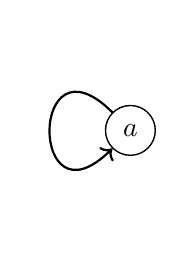
\begin{tikzpicture}
        \GraphInit[vstyle=normal]
        \SetGraphUnit{1.5}
        \Vertex[Math=true]{a}
        \Loop[dist=1.5cm, style={->}](a)
    \end{tikzpicture}
    \hspace{1em}

    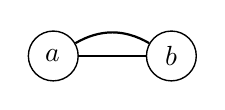
\begin{tikzpicture}
        \GraphInit[vstyle=normal]
        \SetGraphUnit{1.5}
        \Vertex[Math=true]{a}
        \EA[Math=true](a){b}
        \Edge[style={-, bend left}](a)(b)
        \Edge[style={-}](a)(b)
    \end{tikzpicture}
    \caption{环(上)与多重边(下)}
    \label{fig:环与多重边}
\end{figure}

如果一个图不存在多重边或者环,那么该图被称为简单图;如果一个图存在多重边和环,那么该图被称为伪图;如果一个图存在多重边但不存在环,那么该图称为多重图。

\begin{table}[H]
    \centering
    \begin{tabular}{ccc}
        \toprule
        \makebox[2cm][c]{多重边} & \makebox[2cm][c]{环} & \makebox[2cm][c]{类型} \\
        \midrule
        不存在 & 不存在 & 简单图 \\
        存在 & 存在 & 伪图 \\
        存在 & 不存在 & 多重图 \\
        \bottomrule
    \end{tabular}
    \caption{简单图、伪图与多重图}
\end{table}

\begin{figure}[H]
    \centering
    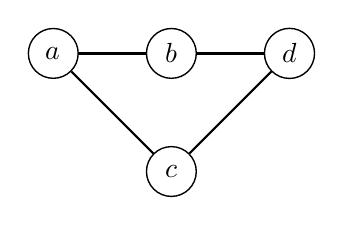
\begin{tikzpicture}
        \GraphInit[vstyle=normal]
        \SetGraphUnit{1.5}
        \Vertex[Math=true]{a}
        \EA[Math=true](a){b}
        \SO[Math=true](b){c}
        \EA[Math=true](b){d}
        \Edge[style={-}](a)(b)
        \Edge[style={-}](a)(c)
        \Edge[style={-}](b)(d)
        \Edge[style={-}](c)(d)
    \end{tikzpicture}
    \hspace{1em}
    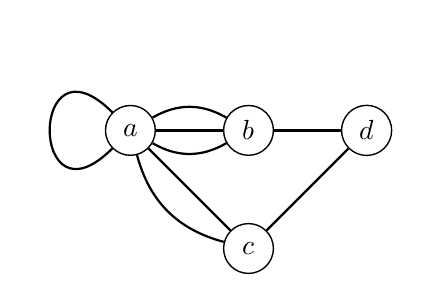
\begin{tikzpicture}
        \GraphInit[vstyle=normal]
        \SetGraphUnit{1.5}
        \Vertex[Math=true]{a}
        \EA[Math=true](a){b}
        \SO[Math=true](b){c}
        \EA[Math=true](b){d}
        \Edge[style={-}](a)(b)
        \Edge[style={-, bend left}](a)(b)
        \Edge[style={-, bend right}](a)(b)
        \Edge[style={-, bend right}](a)(c)
        \Edge[style={-}](a)(c)
        \Edge[style={-}](b)(d)
        \Edge[style={-}](c)(d)
        \Loop[dist=1.5cm, style={-}](a)
    \end{tikzpicture}
    \hspace{1em}
    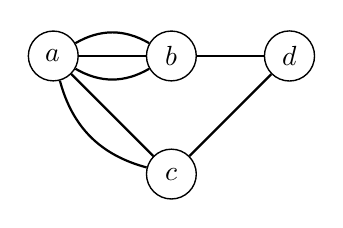
\begin{tikzpicture}
        \GraphInit[vstyle=normal]
        \SetGraphUnit{1.5}
        \Vertex[Math=true]{a}
        \EA[Math=true](a){b}
        \SO[Math=true](b){c}
        \EA[Math=true](b){d}
        \Edge[style={-}](a)(b)
        \Edge[style={-, bend left}](a)(b)
        \Edge[style={-, bend right}](a)(b)
        \Edge[style={-, bend right}](a)(c)
        \Edge[style={-}](a)(c)
        \Edge[style={-}](b)(d)
        \Edge[style={-}](c)(d)
    \end{tikzpicture}
    \caption{简单图(左)、伪图(中)、多重图(右)}
    \label{fig:简单图、伪图与多重图}
\end{figure}

\subsection{完全图、零图与平凡图}
完全图、零图与平凡图都是特殊的无向简单图。完全图指每对不同顶点之间都恰有一条边的简单图;零图指边集为空集的简单图;频繁图指只有一个顶点且边集为空集的简单图。
\begin{figure}[H]
    \centering
    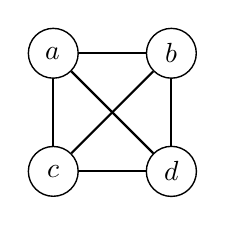
\begin{tikzpicture}
        \GraphInit[vstyle=normal]
        \SetGraphUnit{1.5}
        \Vertex[Math=true]{a}
        \EA[Math=true](a){b}
        \SO[Math=true](a){c}
        \EA[Math=true](c){d}
        \Edge[style={-}](a)(b)
        \Edge[style={-}](a)(c)
        \Edge[style={-}](a)(d)
        \Edge[style={-}](b)(c)
        \Edge[style={-}](b)(d)
        \Edge[style={-}](c)(d)
    \end{tikzpicture}
    \hspace{3em}
    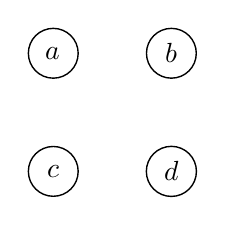
\begin{tikzpicture}
        \GraphInit[vstyle=normal]
        \SetGraphUnit{1.5}
        \Vertex[Math=true]{a}
        \EA[Math=true](a){b}
        \SO[Math=true](a){c}
        \EA[Math=true](c){d}
    \end{tikzpicture}
    \hspace{3em}
    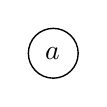
\begin{tikzpicture}
        \GraphInit[vstyle=normal]
        \SetGraphUnit{1.5}
        \Vertex[Math=true]{a}
    \end{tikzpicture}
    \caption{完全图(左)、零图(中)与平凡图(右)}
    \label{完全图、零图与平凡图}
\end{figure}

\subsection{顶点与边的性质}
\begin{definition}[无向图顶点的邻接]\label{def:无向图邻接}
    若 $u$ 和 $v$ 是无向图 $G$ 中的一条边 $e$ 的端点,则称两个顶点 $u$ 和 $v$ 在 $G$ 里邻接,边 $e$ 关联(或连接)$u$ 和 $v$
\end{definition}
\begin{definition}[有向图顶点的邻接]\label{def:有向图邻接}
    若 $(u,v)$ 是有向图 $G$ 中的一条边,则称顶点 $u$ 邻接到 $v$,$v$ 从 $u$ 邻接,$u$ 称为边 $(u,v)$ 的起点,$v$ 称为边 $(u,v)$ 的终点。环的起点与终点相同。
\end{definition}
\begin{definition}[顶点的邻居]\label{def:邻居}
    图 $G=(V, E)$ 中,顶点 $v$ 的所有邻接顶点的集合称为顶点的邻居,记作 $N(v)$。
\end{definition}

\begin{collections}
    \begin{example}
        写出下图中各个顶点的邻居。
            \begin{center}
                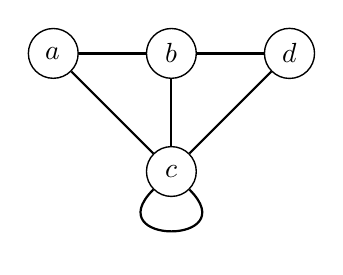
\begin{tikzpicture}
                    \GraphInit[vstyle=normal]
                    \SetGraphUnit{1.5}
                    \Vertex[Math=true]{a}
                    \EA[Math=true](a){b}
                    \SO[Math=true](b){c}
                    \EA[Math=true](b){d}
                    \Edge[style={-}](a)(b)
                    \Edge[style={-}](a)(c)
                    \Edge[style={-}](b)(d)
                    \Edge[style={-}](c)(d)
                    \Edge[style={-}](b)(c)
                    \Loop[dist=1cm, style={-}, dir=SO](c)
                \end{tikzpicture}
            \end{center}
    \end{example}
    \begin{solution}
        \begin{center}
            \begin{tabular}{c|c}
                \toprule
                \makebox[2cm][c]{顶点} & \makebox[2cm][c]{邻居} \\
                \midrule
                $a$ & $b, c$ \\
                $b$ & $a, c, d$ \\
                $c$ & $a, b, c, d$ \\
                $d$ & $b, c$ \\
                \bottomrule
            \end{tabular}
        \end{center}
    \end{solution}
\end{collections}

\begin{definition}[无向图顶点的度]
    无向图中顶点的度是与该顶点相关联的边的数目,如果该顶点存在环,则每个环为顶点的度贡献 $2$。顶点 $v$ 的度记作 $\symrm{deg}(v)$
\end{definition}
\begin{definition}[有向图顶点的出度与入度]
    在有向图中,顶点的出度是以该顶点为起点的边的数目,顶点的入度是以该顶点为终点的边的数目,顶点上的环对出度与入度的贡献均为 1。顶点 $v$ 的出度记为 $\symrm{deg}^+(v)$,顶点 $v$ 的入度记为 $\symrm{deg}^-(v)$。
\end{definition}

如果一个顶点的度为 $0$,那么称其为\textbf{孤立的};如果一个顶点的度为 $1$,那么称其为\textbf{悬挂的}。
\begin{collections}
    \begin{example}
        看下图,求$\symrm{deg}(c)$。
            \begin{center}
                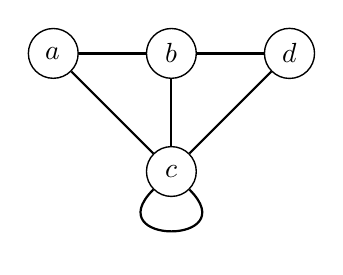
\begin{tikzpicture}
                    \GraphInit[vstyle=normal]
                    \SetGraphUnit{1.5}
                    \Vertex[Math=true]{a}
                    \EA[Math=true](a){b}
                    \SO[Math=true](b){c}
                    \EA[Math=true](b){d}
                    \Edge[style={-}](a)(b)
                    \Edge[style={-}](a)(c)
                    \Edge[style={-}](b)(d)
                    \Edge[style={-}](c)(d)
                    \Edge[style={-}](b)(c)
                    \Loop[dist=1cm, style={-}, dir=SO](c)
                \end{tikzpicture}
            \end{center}
    \end{example}
    \begin{solution}
        $\symrm{deg}(c)=5$
    \end{solution}
    \spare
    \begin{example}
        看下图,求 $\symrm{deg}^+(c)$ 和 $\symrm{deg}^-(c)$。
            \begin{center}
                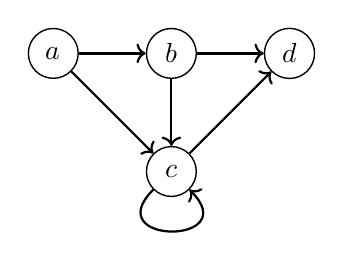
\begin{tikzpicture}
                    \GraphInit[vstyle=normal]
                    \SetGraphUnit{1.5}
                    \Vertex[Math=true]{a}
                    \EA[Math=true](a){b}
                    \SO[Math=true](b){c}
                    \EA[Math=true](b){d}
                    \Edge[style={->}](a)(b)
                    \Edge[style={->}](a)(c)
                    \Edge[style={->}](b)(d)
                    \Edge[style={->}](c)(d)
                    \Edge[style={->}](b)(c)
                    \Loop[dist=1cm, style={->}, dir=SO](c)
                \end{tikzpicture}
            \end{center}
    \end{example}
    \begin{solution}
        $\symrm{deg}^+(c)=2$,$\symrm{deg}^-(c)=3$
    \end{solution}
\end{collections}

\begin{theorem}[无向图的握手定理]\label{thm:无向图的握手定理}
    设 $G=(V,E)$ 是有 $m$ 条边的无向图,则
    \begin{equation*}
        2m = \sum_{v \in V} \symrm{deg}(v)
    \end{equation*}
\end{theorem}
\begin{theorem}[有向图的握手定理]\label{thm:有向图的握手定理}
    设 $G=(V,E)$ 是有 $m$ 条边的有向图,则
    \begin{equation*}
        m = \sum_{v \in V} \symrm{deg}^+(v) = \sum_{v \in V} \symrm{deg}^-(v)
    \end{equation*}
\end{theorem}

握手定理在图中存在环或多重边时依然成立。

由定理 \ref{thm:无向图的握手定理} 可以推得定理 \ref{thm:握手定理推论}。
\begin{theorem}\label{thm:握手定理推论}
    无向图有偶数个度为奇数的顶点。
\end{theorem}

\begin{collections}
    \begin{example}
        如果一个无向图中有 6 个顶点,每个顶点的度均为 10,则该图中有多少条边?
    \end{example}
    \begin{solution}
        设该图为 $G=(V, E)$,有 $m$ 条边,由题意可知

        $$\sum_{v \in V}\symrm{deg}(v) = 6 \times 10 = 60$$

        由握手定理可知

        $$\sum_{v \in V}\symrm{deg}(v) = 2m$$

        则

        $$2m = 60$$

        解得 $m=30$

        综上所述,该图有 $30$ 条边。
    \end{solution}
\end{collections}

\subsection{子图与并图}
\begin{definition}[子图]\label{def:子图}
    设图 $G=(V, E)$ 与图 $H=(W, F)$ 存在 $W \subseteq V$ 与 $E \subseteq F$,则称图 $H$ 是图 $G$ 的子图,记作 $H \subseteq G$。
\end{definition}
\begin{definition}[真子图]\label{def:真子图}
    设图 $G=(V, E)$ 与图 $H=(W, F)$ 存在 $W \subseteq V$ 与 $E \subseteq F$,且$H \neq G$,则称图 $H$ 是图 $G$ 的真子图,记作 $H \subsetneqq G$。
\end{definition}
\begin{definition}[生成子图]\label{def:生成子图}
    设图 $G=(V, E)$ 与图 $H=(W, F)$ 存在 $W = V$ 与 $E \subseteq F$,则称图 $H$ 是图 $G$ 的生成子图。
\end{definition}

显然,任意图 $G$ 都是自身的子图。
\begin{figure}[htbp!]
    \centering
    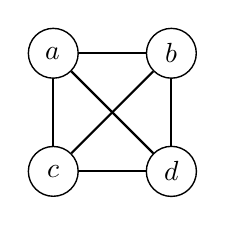
\begin{tikzpicture}
        \GraphInit[vstyle=normal]
        \SetGraphUnit{1.5}
        \Vertex[Math=true]{a}
        \EA[Math=true](a){b}
        \SO[Math=true](a){c}
        \EA[Math=true](c){d}
        \Edge[style={-}](a)(b)
        \Edge[style={-}](a)(c)
        \Edge[style={-}](a)(d)
        \Edge[style={-}](b)(c)
        \Edge[style={-}](b)(d)
        \Edge[style={-}](c)(d)
    \end{tikzpicture}
    \hspace{3em}
    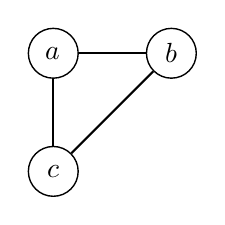
\begin{tikzpicture}
        \GraphInit[vstyle=normal]
        \SetGraphUnit{1.5}
        \Vertex[Math=true]{a}
        \EA[Math=true](a){b}
        \SO[Math=true](a){c}
        \Edge[style={-}](a)(b)
        \Edge[style={-}](a)(c)
        \Edge[style={-}](b)(c)
    \end{tikzpicture}
    \hspace{3em}
    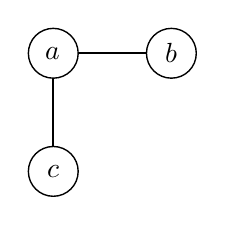
\begin{tikzpicture}
        \GraphInit[vstyle=normal]
        \SetGraphUnit{1.5}
        \Vertex[Math=true]{a}
        \EA[Math=true](a){b}
        \SO[Math=true](a){c}
        \Edge[style={-}](a)(b)
        \Edge[style={-}](a)(c)
    \end{tikzpicture}
    \hspace{3em}
    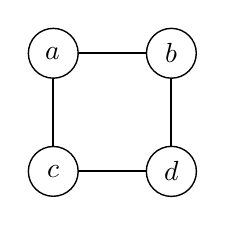
\begin{tikzpicture}
        \GraphInit[vstyle=normal]
        \SetGraphUnit{1.5}
        \Vertex[Math=true]{a}
        \EA[Math=true](a){b}
        \SO[Math=true](a){c}
        \EA[Math=true](c){d}
        \Edge[style={-}](a)(b)
        \Edge[style={-}](a)(c)
        \Edge[style={-}](b)(d)
        \Edge[style={-}](c)(d)
    \end{tikzpicture}
    \caption{图 $G$(左一) 与他的子图(左二)、真子图(右二)、生成子图(右一)}
    \label{fig:子图、真子图与生成子图}
\end{figure}


\end{document}